\documentclass[
    corpo=11.5pt,
    oneside,
    evenboxes,
    tipotesi=triennale,
    stile=classica,
    oldstyle,
    autoretitolo,
    greek,
]{toptesi}
\usepackage[utf8]{inputenc}
\usepackage[T1]{fontenc}
\usepackage{lmodern}
\usepackage{hyperref}
\usepackage{setspace}
\usepackage{verbatim}
\usepackage{pgfplots}
\usepackage{graphicx}
\usepackage{subfig}
\onehalfspacing

\hypersetup{
    pdfpagemode={UseOutlines},
    bookmarksopen,
    pdfstartview={FitH},
    colorlinks,
    linkcolor={blue},
    citecolor={blue},
    urlcolor={blue}
  }
\usepackage{lipsum}

\newtheorem{osservazione}{Osservazione}

\begin{document}\errorcontextlines=9

\begin{ThesisTitlePage}
    \ateneo{Universit\`a degli Studi di Torino}
    \StrutturaDi{Dipartimento di Management}
    \struttura[]{}
    \NomeElaborato{Tesi di laurea triennale}
    \titolo{Lo stato di salute del Calcio}
    \sottotitolo{Fair Play Fiananziario e Superlega}     
    \corsodistudi{Management dell'Informazione e della Comunicazione Aziendale}
    \candidato{Riccardo \textsc{Borgo}}
    \relatore{prof.ssa ~Simona \textsc{Alfiero}}
    \sedutadilaurea{\textsc{Anno~accademico} 2021-2022}
    \logosede{img/Unito-logo, img/logo_saa.jpeg}
\end{ThesisTitlePage}

\tablespagetrue\figurespagetrue
\indici

\mainmatter
\begin{interlinea}{1.5}
    
\chapter{Introduzione generale}
Durante lo sviluppo di questa trattazione si andrà ad analizzare l'attuale "stato di salute"
del calcio europeo, di come il \emph{Financial Fair Play} abbia provato da una parte ad aiutare le società a rimanere in regola con i conti e 
dall'altra a dettare delle regole atte ad evitare comportamenti illegali da parte sopratutto dei presidenti.\\
Infine si tratterà il caso della \emph{Superlega}, per cercare di capire se questa nuova idea sia effettivamente coerente con l'epoca in cui stiamo vivendo.\\
Sopratutto a partire dall'inizio della pandemia da COVID-19 nei primi mesi del 2020 il mondo del calcio si è visto ridurre sensibilmente i ricavi, non riuscendo 
ancora oggi ad operare al 100\%. Grazie, forse, a questa situazione di difficoltà è stato evidenziato come la situazione odierna non fosse più sostenibile: 
club con milioni di euro di debiti, richieste di ingaggio "faraoniche" da parte dei calciatori, con il risultato che molte societ\`a non sono state pi\`u in grado di far fronte 
a tutto questo e costrette a dichiarare falimento.\\
Il primo capitolo mira ad analizzare la situazione economica, finanziaria e patrimoniale, antecedente all'anno 2020 di alcune delle più 
importanti e storiche societ\`a di tutto il panorama europeo: Juventus per quanto riguarda l'Italia, Paris Saint Germain per quanto riguarda la 
Francia, Bayern Monaco per la Germania, Manchester City per l'Inghiterra e il Barcellona per la Spagna. I punti principali dell'analisi riguarderanno: 
Analisi dei ricavi, Analisi della liquidit\'a, Analisi della solidit\'a, Analisi della redditivit\'a e Trend azionario (se presente) in modo da 
poter fare una verifica a 360° di tutti i vari settori economici. La scelta \'e virata su queste societ\'a perch\'e per un motivo o per un altro sono state 
al centro di problematiche o scandali legate alla cattiva gestione del patrimonio oppure "accusate" di non essere state prese particolarmente prese di mira dalle misure e le leggi 
emanate nell'ultimo decennio dalla UEFA \footnote{ Union of European Football Associations}, come per esempio il \emph{Financial Fair Play}.\\
Il secondo capitolo si occuper\'a invece della presentazione e dell'analisi in modo dettagliato del \emph{Financial Fair Play} o 
\emph{FFP}, dalla sua nascita, alle varie parti presenti all'interno del documento e mostrando infine come, non sempre, tutte le societ\'a siano state trattate allo stesso modo.\\
Il terzo capitolo invece analizza invece l'impatto mediatico, non prima di aver presentato tutti i dati tecnici, di una delle ultime novità 
del mondo del calcio: la \emph{Superlega}: il nuovo modello che punta a rivoluzionare il mondo del calcio, per cercare di uscire da questa spirale di debiti
e fallimenti per cercare quindi di creare un nuovo inizio. Verr\'a mostrato in seguito se il progetto ha effettivamente preso piede all'interno del mondo del calcio 
e se è riuscito a smuovere qualcosa, portando agli occhi di tutti l'insostenibilità del modello attuale.\\
In chiusura si cercherà di determinare se i rimedi proposti dalle autorità del mondo del calcio siano stati sufficienti ad eliminare tutte le criticità presenti e 
sopratutto evidenziare l'impatto economico di questi rimedi.\\
Riuscir\'a la Superlega ad acquistare credibilità e ad affermarsi come nuovo modello, capace di risollevare il calcio?

\part{Parte Prima}
\chapter{Situazione economica Europea pre-pandemia da COVID19}
\section{Analisi generale delle diverse realt\'a Europee}
Prima di andare ad analizzare nello specifico i vari club europei \'e necessario iniziare con una prima 
parte atta a presentare la situazione generale all'interno di ogni Paese. Verrà mostrato come non in tutti 
si riesca ad arrivare ad un risultati positivo, andando quindi a rendere in qualche modo 
"unico" ogni campionato e la sua relativa Federazione. Le Federazioni (uniche per ogni Stato) hanno tendenzialmente il compito
comune di organizzare i campionati nazionali e designare gli arbitri per i vari incontri. Oltre a questo compito pi\'u di tipo
organizzativo le varie Federazioni hanno il dovere di garantire un accesso libero ed universale al gioco del calcio, senza distinzioni
di genere ed etnia. Questi due compiti \'e possibile estrapolarli dagli 11 punti contenenti i valori che la UEFA 
\footnote{Wikipedia: Union of European Football Associations, raggruppa tutte le Federazioni dei vari stati Europei e non} vuole
trasmettere tramite la sua attivit\'a \footnote{Wikpedia: https://it.wikipedia.org/wiki/Union\_of\_European\_Football\_Associations, I Valori UEFA}.\\
L'analisi verter\'a principalmente su due settori: \textbf{risultato economico 2019} e \textbf{analisi degli stipendi}; questi due elementi
permettono di generare un'opinione abbastanza completa perch\'e da un lato si evidenzier\'a come si \'e giunti a quel risultato (entrate e spese)
e dall'altra si analizzer\'a uno dei temi pi\'u discussi di sempre riguardo il mondo del calcio, andando a capire se gli stipendi dei calciatori
siano collegati o meno ai risultati ottenuti.

\subsection{Italia}
Questa prima analisi inizia con l'Italia. Il Paese, dal punto di vista calcistico, \'e gestito dalla FIGC \footnote{Federazione Italiana Giuoco Calcio}
che non sempre si \'e rivelata del tutto limpida nella gestione: il caso pi\'u eclatante \'e sicuramente lo scandalo \emph{Calciopoli} del
2005 in cui risult\'o coinvolto anche l'allora presidente Franco Carraro e vicepresidente Innocenzo Mazzini \footnote{Wikipedia: https://it.wikipedia.org/wiki/Calciopoli}.
Vi \'e quindi da molti anno una sorta di diffidenza nei contronti della federazione, con ancora oggi molti dubbi sulla presenza o meno di 
corruzione al suo interno.\\
Il tema dell'analisi, come prima spiegato, non sar\'a per\'o questo.\\
Iniziando con il primo tema la figura \ref{ris_italia} mostra come il Risultato Netto consolidato di tutti e tre i campionati 
sotto la FIGC, dato dalla somma algebrica delle voci precedenti, sia fortemente negativo con un valore che si attesta 
a -395mln€ \footnote{FIGC: https://www.figc.it/it/federazione/federazione-trasparente/reportcalcio/} confermando un trend negativo che
si interrompre solo nel 2016/2017.
Il valore che pi\'u incide su questo risultato sono gli ammortamenti e svalutazioni che, sommati ai costi di produzione, 
annullano completamente i ricavi generati. 
\begin{figure}
    \centering
    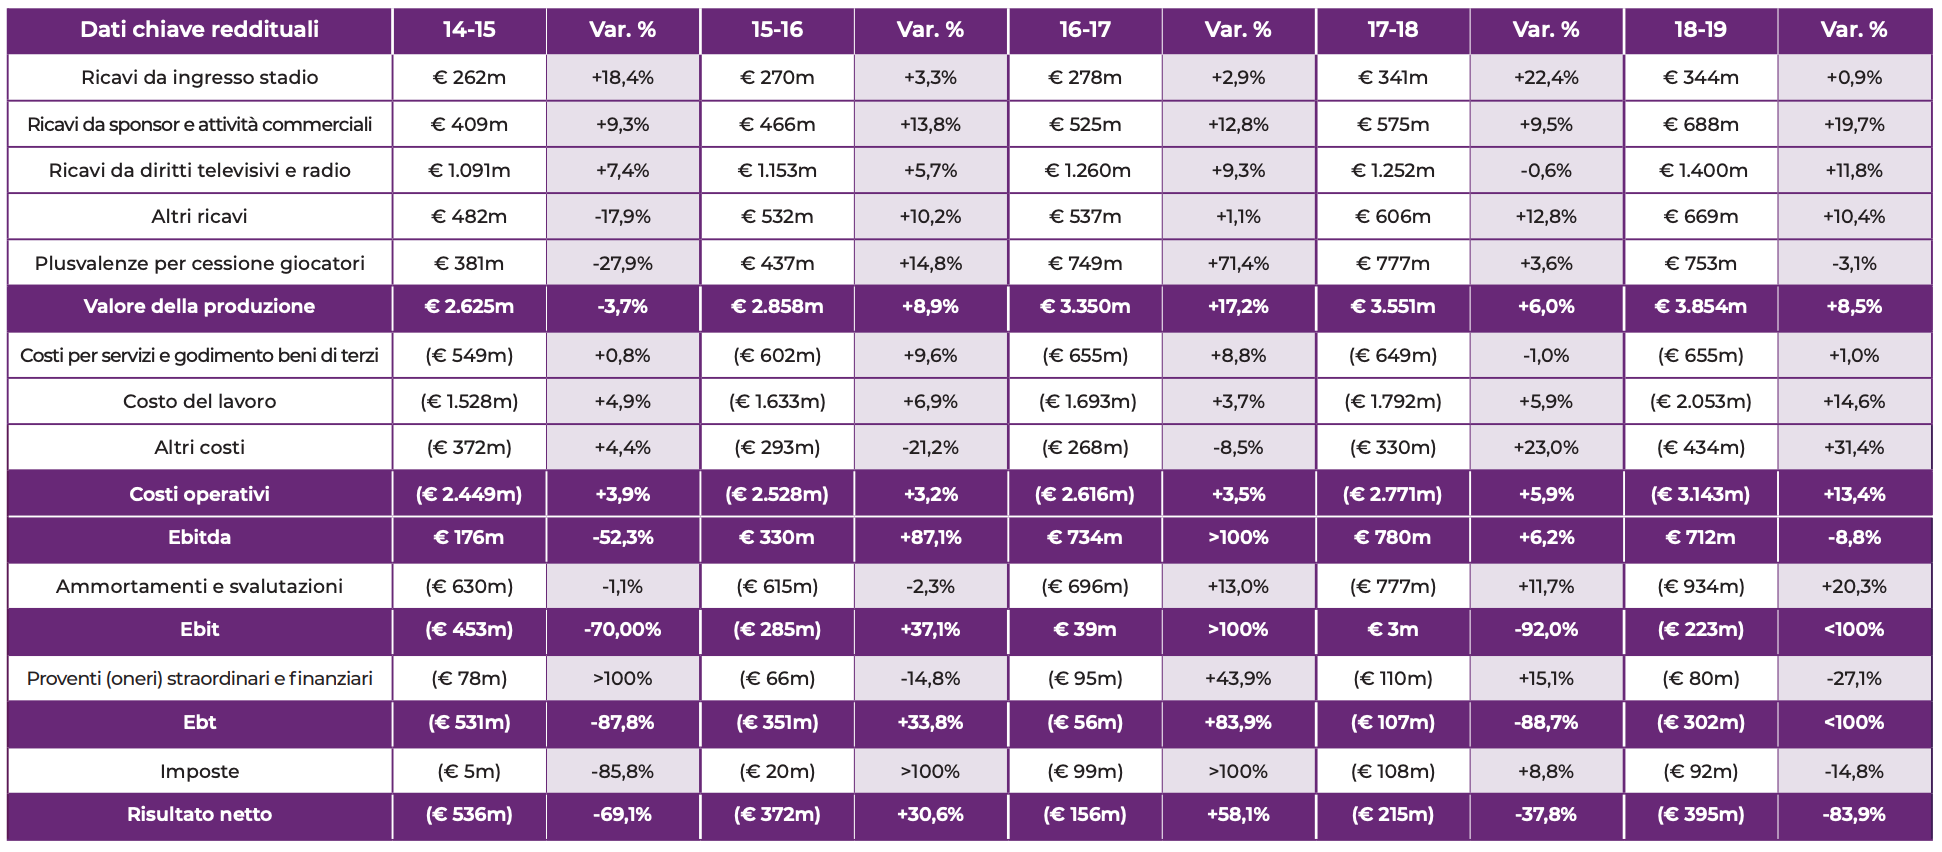
\includegraphics[scale=0.4]{img/ris_italia.png}
    \caption{Principali risultati del campionato di Serie A 2018/2019}
    \label{ris_italia}
\end{figure}
All'interno del mondo del calcio gli ammortamenti sono riferiti ai calciatori e al loro prezzo di acquisto perch\'e sono considerati delle 
vere e proprie immobilizzazioni, con un costo storico (prezzo di acquisto) e vita utile (durata del contratto). 
Come mostra la figura questo valore ha subito un incremento costante a partire dal 2013, il che non \'e necessariamente un male, perch\'e 
sta a significare che le societ\'a investono nei calciatori per cercare risultati sempre migliori; se per\'o questi risultati non vengono
raggiunti i costi non saranno coperti dai ricavi, andando quindi a generare una perdita. L'unico modo per permettere ad un Paese di crescere
caocisticamente \'e tramite la vittoria di competizioni internazionali, quali la UEFA Champions League oppure la UEFA Europa League, che
elargiscono premi importanti. Tuttavia, a partire dalla stagione 2013/2014 ci sono stati ben pochi risultati soddisfacenti 
da parte delle squadre italiane in Europa: gli unici risultati degni di nota sono le due finali giocate da parte della Juventus in 
Champion League (14/15 e 16/17) e una semifinale raggiunta dalla Roma nella Champions League 17/18. Questi risultati, per quanto importanti,
non hanno permesso di far fronte ai sempre maggiori aumenti dei costi per cercare di vincere queste competizioni, uno su tutti l'acquisto
di Cristiano Ronaldo da parte della Juventus dal Real Madrid nell'estate 2019 per la cifra di 115mln€ di cartellino e 57mln€ di stipendio (lordo) annuo
\footnote{Eurosport: https://www.eurosport.it/calcio/calciomercato/2017-2018/cristiano-ronaldo-juventus-costo-contratto-e-stipendio-tutti-i-dettagli-dell-affare\_sto6841703/story.shtml}.\\
\subsection{Francia}
Per quanto riguarda invece la Francia, l'organizzazione che si occupa del monitoraggio e la supervisione dei conti 
delle società calcistiche di associazioni di calcio in Francia è la DNCG \footnote{Direction Nationale du Contrôle de Gestion}. Essa 
pubblica ogni stagione un report riassuntivo per quanto riguarda la Ligue 1 e la Ligue 2 (i primi due campionati francesi) ed una
relazione relativa ad ogni singolo club dei due campionati. Tutti i dati di seguito riportati sono stati reperiti dai singoli
report annuali pubblicati \footnote{https://www.lfp.fr/dncg/rapports} \\
I risultati della stagione appena conclusa vengono riassunti con la figura \ref{ris_generali_2019}:
\begin{figure}
    \centering
    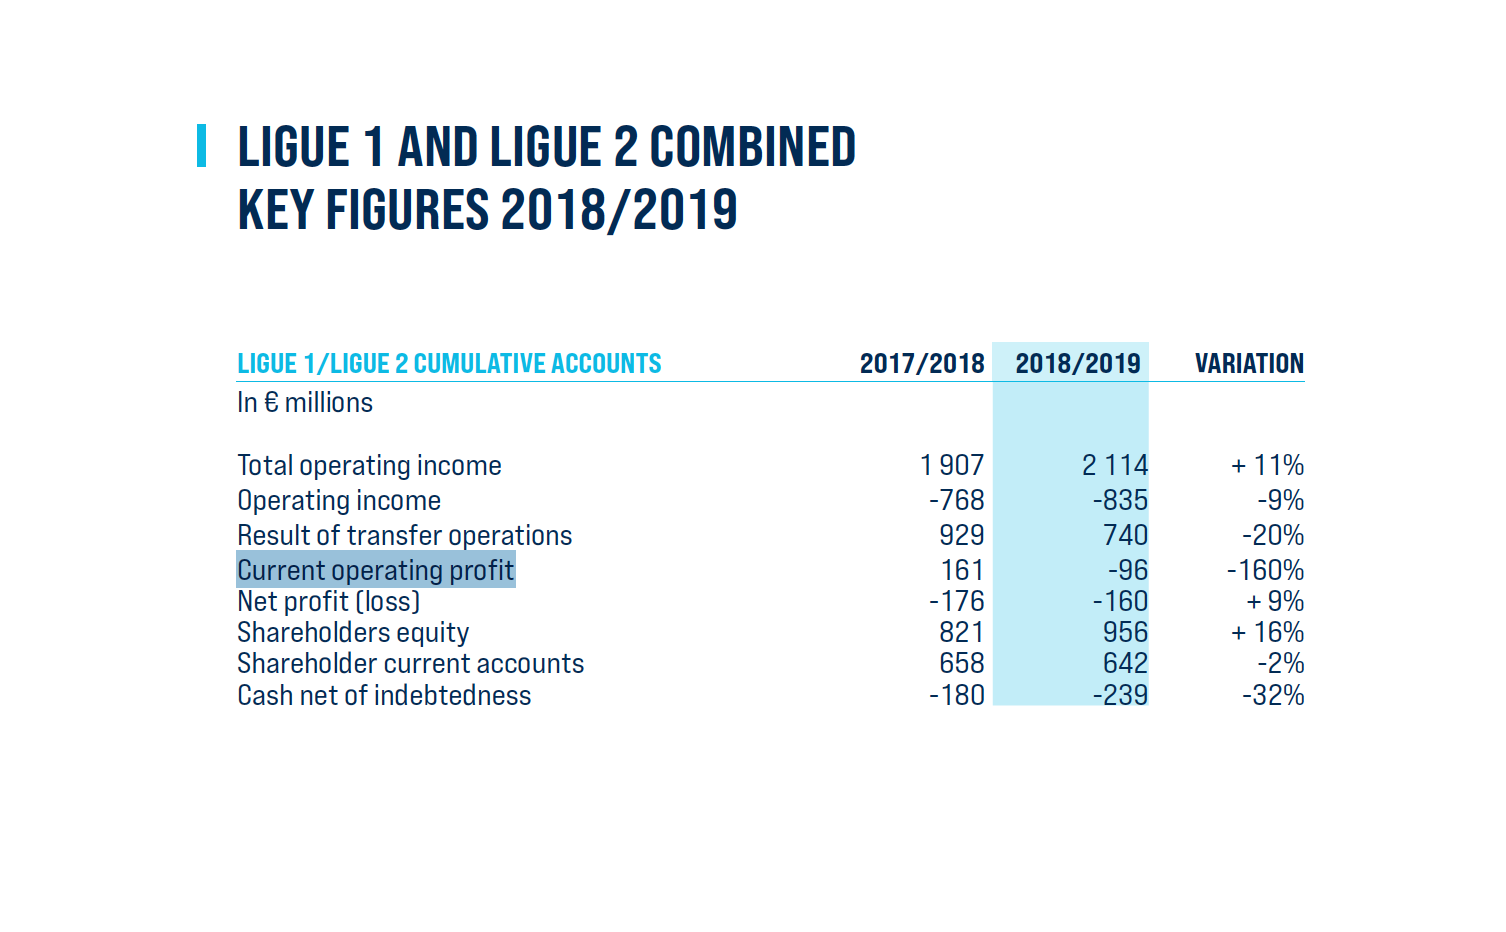
\includegraphics[scale=.5]{img/ris_generali_2019}
    \caption{Risultati generali combinati 2018/2019}
    \label{ris_generali_2019}
\end{figure}
Al termine della stagione 2018/2019 il risultato netto "consolidato" ammontava a -160 mln€, in miglioramento per\'o del 9\% rispetto 
all'anno prima (-176). Questo risultato, come indicato prima, \'e il risultato della sottrazione tra ricevi e costi d'esercizio
dei due campionati; andando ad analizzare 
nello specifico i due risultati \'e possibile notare come la Ligue 1 abbia osservato un incremento del 20\% del risultato netto
consolidato rispetto alla stagione precedente ma la Ligue 2 ha dovuto affrontare un calo del 90\% del Net Profit, andando quindi completamente
ad annullare il risultato positivo del campionato superiore. Questo risultato molto negativo \'e spiegabile tramite la comparazione 
dei grafici che mostrano la composizione del Net Income nella stagione 18/19 e precedente mostrato nella figura \ref{comp_income}.
\begin{figure}
    \centering
    \subfloat[][Composizione Net Income stagione 2017/2018]
    {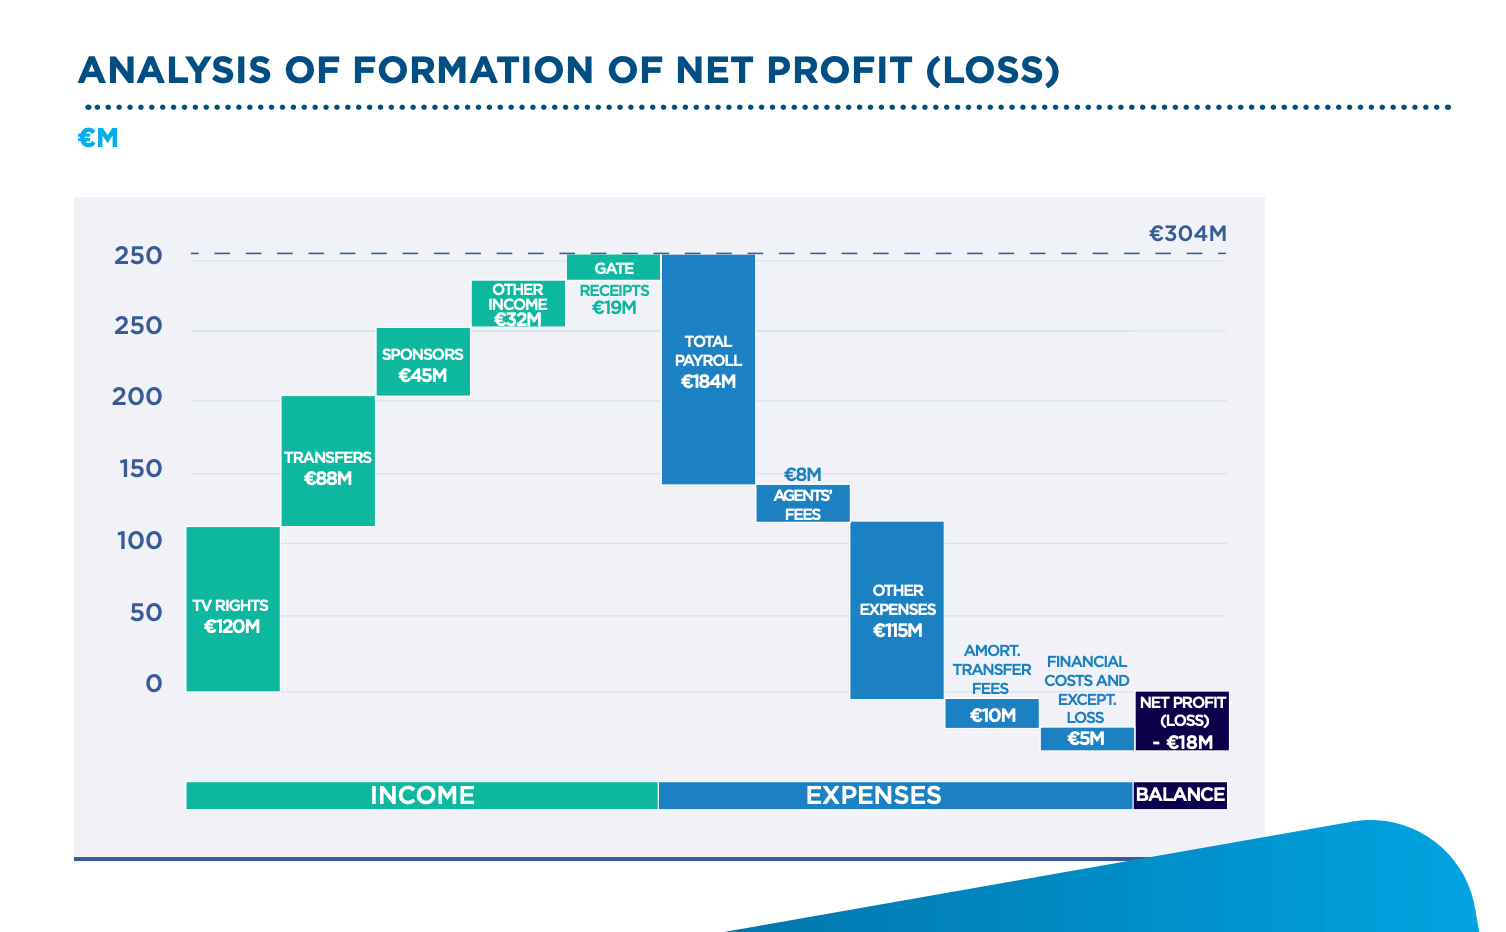
\includegraphics[width=.45\textwidth]{img/net_income_2018.png}} \quad
    \subfloat[][Composizione Net Income stagione 2017/2018]
    {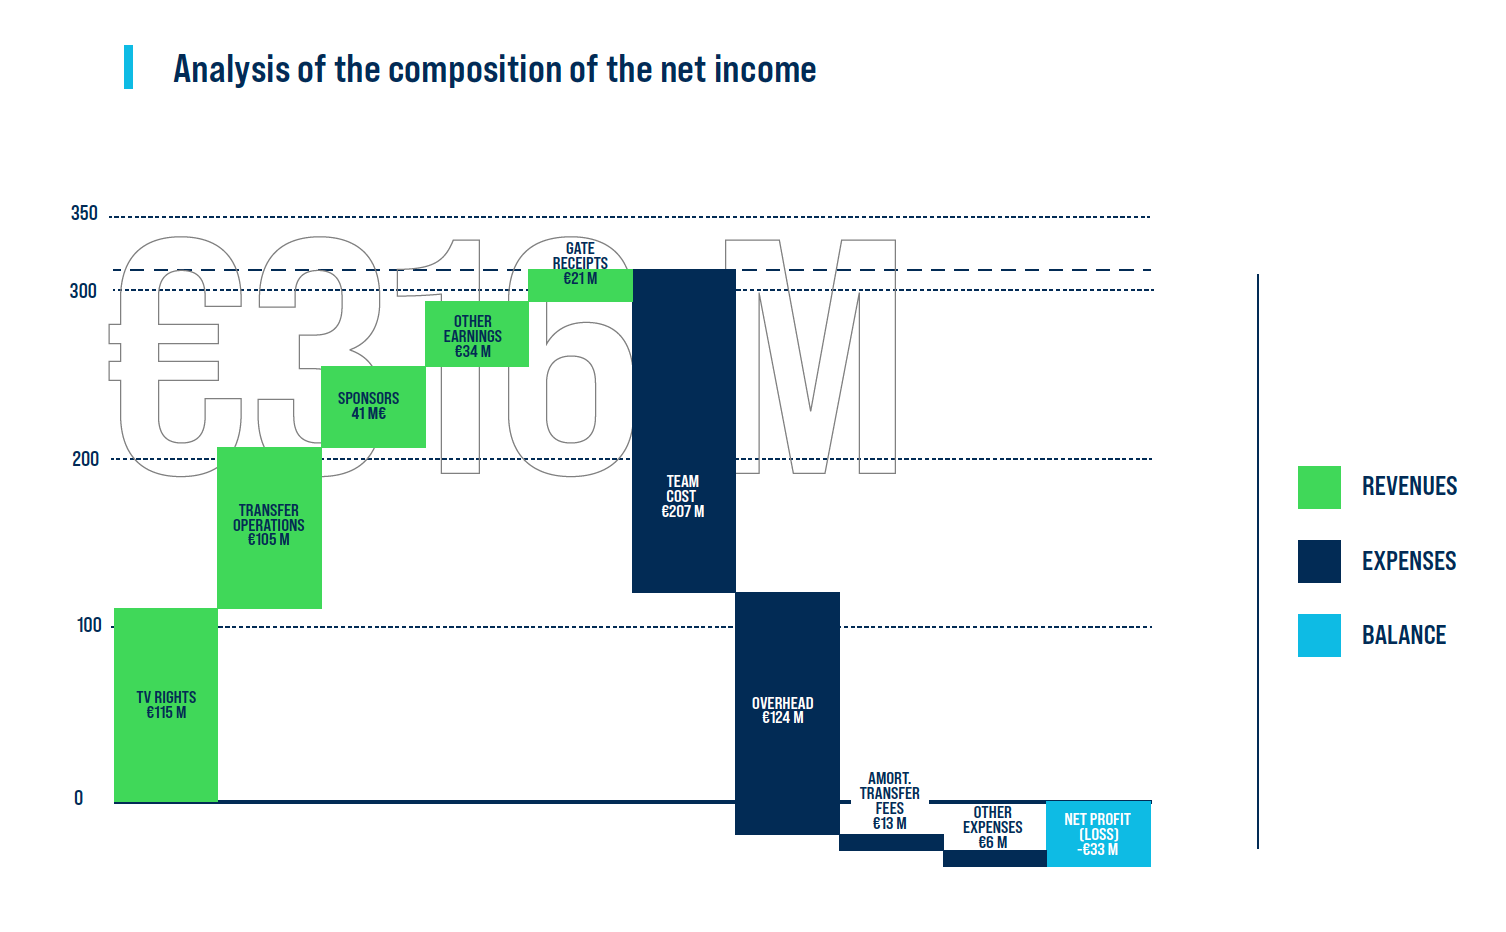
\includegraphics[width=.45\textwidth]{img/net_income_2019.png}}
    \caption{Comparazione Risultato Netto (Net Income)}
    \label{comp_income}  
\end{figure}

La perdita registrata nella stagione 18/19 \'e la seconda in termini di importanza a partire dalla stagione 2013/2014 e
il motivo principale che spiega questa discesa cos\'i decisa, \'e da attribuirsi ad un aumento delle entrate (\emph{Income}),
con un valore che passa da 304 mln€ nel 17/18 a 316 mln€ nel 18/19, che per\'o non riesce a controllare l'aumento pi\'u considerevole
delle spese (\emph{Expenses}), sopratutto nella parte dedicata alle spese dei club (stipendi di giocatori e commissioni degli agenti) 
e nella parte delle "Altre spese" (\emph{Other Expenses}) che aumentano rispettivamente di 5 e 9 mln€. Inoltre, osservando le due figure,
si pu\'o notare come nella prima stagione la parte di spese relativa ai club e la voce "Altre spese" andasse a portare a 0 il profitto,
mentre nella stagione successiva gi\'a solo queste due voci vanno a creare una perdita.\\
Un secondo indicatore che \'e possibile prendere in considerazione per questa prima analisi generale \'e il \emph{Payroll}. Con questo termine
si esprime lo stipendio anno di un club ed occupa vari punti all'interno dell'analisi pubblicata da DNCG. Nel nostro caso prendiamo 
in considerazione la figura \ref{stipendi_ligue1} che esprime il Payroll medio dei club a seconda della posizione che hanno raggiunto
in classifica nella stagione 2018/2019. \'E possibile notare immediatamente come la differenza tra le squadre qualificate per 
la Uefa Europa League e quelle che hanno raggiunto la Uefa Champions League abbiano una differenza di Payroll medio di 75,9 mln€ 
che, considerando la differenza di posizionamento in classifica (in generale massimo 3 posizioni), \'e un valore molto elevato. 
Sicuramente la colonna pi\'u a destra \'e composta in modo considerevole dalla squadra Paris Saint Germain 
(oggetto di una trattazione successiva) che, grazie ai fondi Arabi, possono permettersi
stipendi di gran lunga maggiori della media rispetto alle altre squadre del campionato.
\begin{figure}
    \centering
    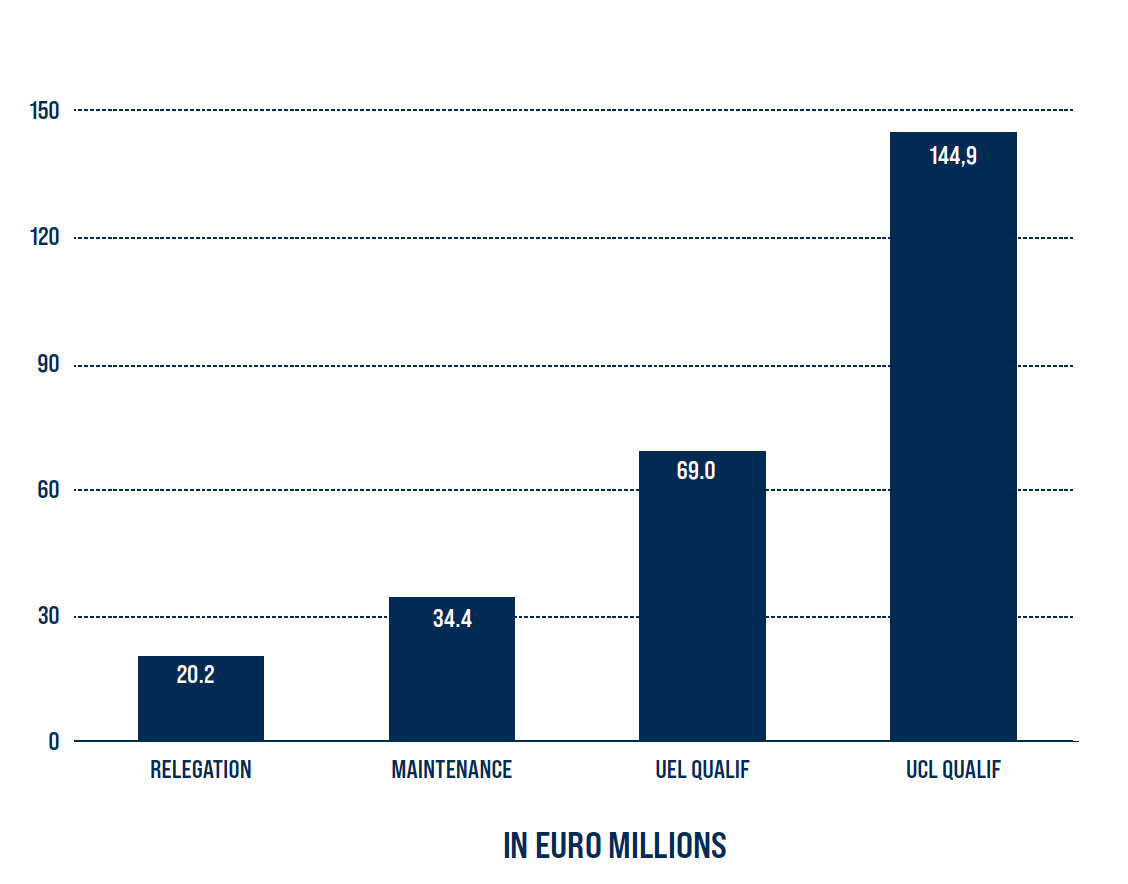
\includegraphics[scale=.5]{img/stipendi_ligue1.png}
    \caption{Stipendio medio dei club che occupano rispettivamente le diverse zone della classifica: zona retrocessione, 
    mat\'a classifica, qualificazione per Uefa Europa League e qualificazione per Champions League}
    \label{stipendi_ligue1}
\end{figure}

Nonostante un Payroll, almeno per quanto riguarda le squadre qualificate per la UCL \footnote{Uefa Champions League}, in linea con gli
altri campionati (147 mln€ nella Premier League inglese \footnote{Calcolo personale utilizzando i dati da https://www.spotrac.com/epl/payroll/})
i risultati ottenuti nelle competizioni internazionali non sono state all'altezza; nella stagione 2018/2019 sono presenti 3 squadre 
all'interno della fase a gironi della massima competizione europea: Monaco, Paris Saint Germain e Olympique Lione. La prima si 
posizione ultima nel gruppo A, la seconda (da cui gli esperti e i sostenitori si aspettano grandi risultati, visti i milioni di euro 
spesi ogni anno) viene eliminata agli ottavi di finale e infine la terza viene anch'essa eliminata agli ottavi di finale. Questo scenario
si ripete mediamente ogni anno, mentre, se si vuole trovare una squadra francese vincitrice dobbiamo tornare indietro alla stagione 1992/1993
con l'Olympique Marsiglia.\\
Ripartendo dall'ultimo indicatore analizzato e collegandolo al primo \'e possibile constatare come i grandi investimenti spesso non portano 
al successo assicurato e quindi ad un ritorno concreto. Queste grosse somme che escono dalle casse dei club che per\'o
non vedono un ritorno portano un danno a tutto il campionato, perch\'e da un lato viene aumentato il gap tecnico tra le diverse squadre dello
stesso campionato mentre dall'altro, in campo internazionale, non si ottengono risultati non ricevendo quindi premi da sponsor e organizzatori.
Tutto questo circolarit\'a non fa' altro che danneggiare il sistema calcio francese perch\'e si fa perdere valore e quindi appeal, sia 
visivo che economico, al campionato locale e si "danneggia" l'immagine europea dei club francesi, considerati incapaci nonostante le somme spese
di ottenere risultati.

\subsection{Germania}
Come terzo elemento sui cinque totali campionati presi in esame in questa introduzione si andr\'a ad approfondire la situazione
in Germania. Per la prima volta sar\'a possibile evidenziare molti aspetti positivi perch\'e questo campionato, come pochi in Europa,
ho davvero pochi punti critici, questo grazie forse al tipo di societ\'a, quella Tedesca, molto piu\'u serie e concentrata rispetto
ad altre realt\'a.\\
Come primo elemento si \'e deciso di analizzare il risultato che pi\'u di tutti viene pubblicizzato da parte della Lega stessa: 
4.02 mld€ di ricavo generato solamente dalla Bundesliga (primo campionato nazionale) in un solo anno,
considerabile un grande traguardo raggiunto e che rimane un primato da 15 anni consecutivi
\footnote{https://www.dfl.de/en/2018-dfl-report/}.

\begin{figure}
    \centering
    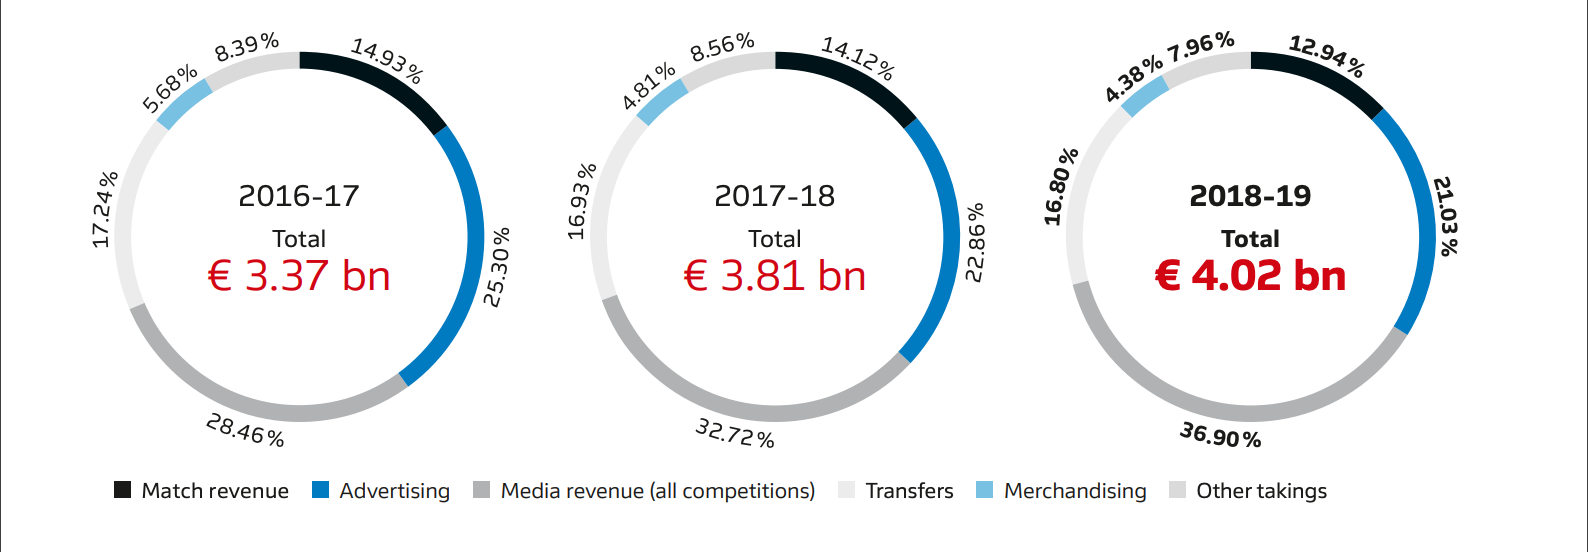
\includegraphics[scale=.5]{img/bundes_entrate.png}
    \caption{Ricavi totali Bundesliga e 2.Bundesliga dal 2012/2013 al 2018/2019}
    \label{entrate_bundes}
\end{figure}
Come mostra la figura \ref{entrate_bundes} le entrate del primo campionato in Germania sono cresciute da 3.37 mld€ nel 2016/2017
a, come detto in precedenza, 4.02 mld€ nel 2018/2019, registrando quindi un incremento del 19.3\% circa. Entrando nel dettaglio, sono aumentati
anche i ricavi dai media grazie ai maggiori contratti nazionali siglati dalla stagione precedente tuttavia sono diminuiti, anche se di poco,
i ricavi da pubblicit\'a e incontri, imputabile in modo prevalente ad un cambio della composizione del campionato stesso.


Dopo aver presentato questi dati \'e possibile formulare un giudizio sui risultati registrati dal settore calcio in Germania: all'interno
di questo Stato vige Sicuramente una cultura legata alla precisione e al rispetto sia delle leggi che delle persone, questo si riflette 
ovviamente in tutti gli ambiti compreso quello del calcio. Come \'e possibile notare, in questo caso, i club prestano molta attenzione a non 
terminare l'anno economico con elevati debiti oppure con risultati ad un passo dal fallimento, nonostante questo arrivano anche risultati dal 
campo perch\'e negli ultimi anni le squadre tedesche sono sempre riuscite a ritagliarsi il proprio spazio nelle competizioni europee, 
culminato con la vittoria della Champions League da parte del Bayern Monaco nel 2020. 

\subsection{Spagna}
Come penultimo campionato oggetto dell'analisi troviamo il campionato spagnolo, formato dalla prima divisione La Liga Santander e la seconda
La Liga Smartbank. Come per il campionato tedesco precedentemente analizzato verr\'a preso in esame il Total Income come punto di partenza
\footnote{Tutti i dati provengono da: https://www.laliga.com/en-GB/transparency/economic-management/economic-report}.
La figura \ref{total_income_spain} permette di visualizzare all'istante come il Reddito Complessivo dei due campionati sia in crescita 
dalla stagione 2013/2014. Si parte con un valore combinato di 2688.5 mln€ e si arriva alla stagione 18/19 con un totale di 4871.4 mln€, 
un'incremento dell'81,19\%. 
\begin{figure}
    \centering
    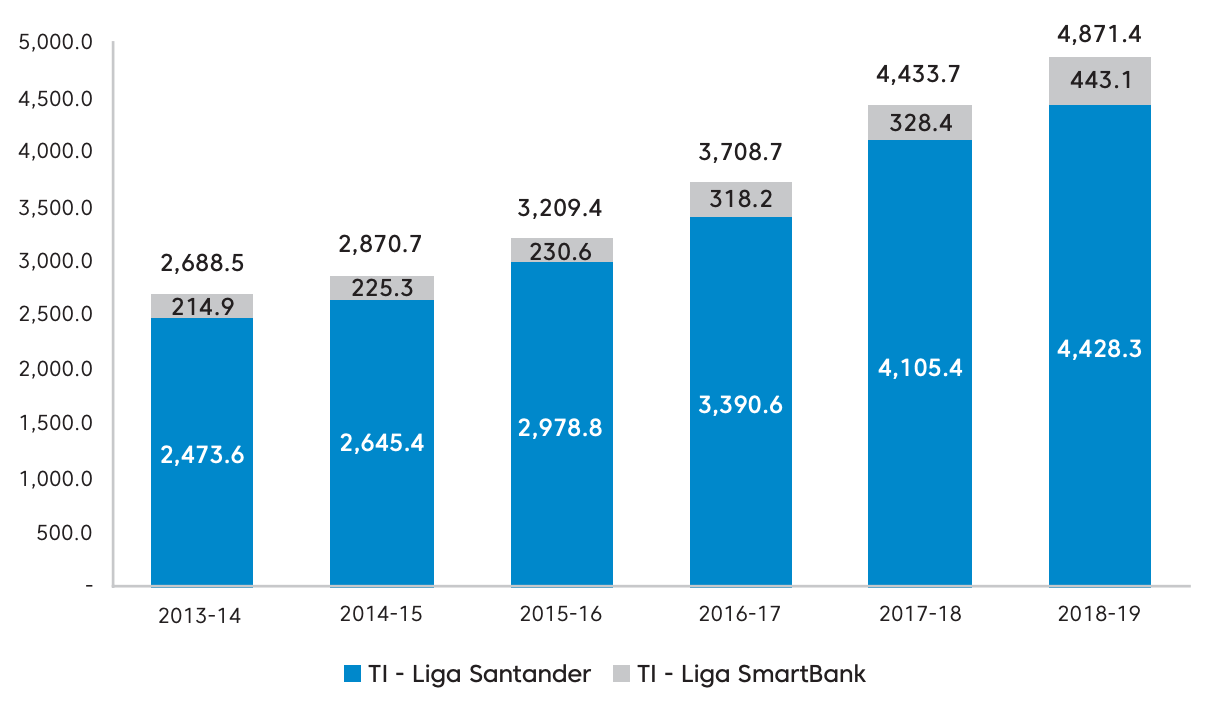
\includegraphics[scale=0.5]{img/total_income_spain.png}
    \caption{Reddito Complessivo per la Liga Santander (Blu) e per la Liga SmartBank (grigio)}
    \label{total_income_spain}
\end{figure}
Suddividendo in modo settoriale il Total Income \'e possibile capire come in tutti i settori si sia verificato un aumento rispetto agli anni
precedenti, andando a mostrare quindi come il campionato spagnolo abbia vissuto una forte crescita negli ultimi 6 anni.
I diversi settori sono:
\begin{enumerate}
    \item \textbf{Trasmissioni}: 1665.1 mln€ (+6.2\% rispetto all'anno precedente e +13.6\% in 5 anni). Questa crescita \'e dovuta sopratutto ad una distribuzione 
    centralizzata dei diritti grazie al RDL 5/2015 \footnote{Wikipedia: Real Decreto Ley è un atto avente forza di legge emanato dal Re}.
    \item \textbf{Attivit\'a commerciali}: 983.8 mln€ (+5.5\% rispetto all'anno precedente e +16.7\% in 5 anni). Comprende sponsorizzazioni,
    pubblicit\'a e merchandising.
    \item \textbf{Partite}: 948.6 mln€ (+24.4\% rispetto all'anno precedente e +9.3\% in 5 anni). Comprende le competizioni, biglietti 
    e altre entrate distribuite dalla UEFA.
\end{enumerate}
Il risultato finale del Reddito \'e stato in modo importante favorito dalla crescita di altri 2 fattori che caratterizzano l'attivit\'a del
campionato:
\begin{enumerate}
    \item \textbf{Trasferimenti}: 1,006.2 mln€ (+7.2\% rispetto all'anno precedente e +18.1\% in 5 anni).
    \item \textbf{ALtre Entrate}: : 267.7 mln€ (+15.7\% rispetto all'anno precedente e -2.8\% in 5 anni). Unico valore che vede una diminuzione
    nel medio periodo ma dovuta al fatto che questa voce, comprendendo accordi di natura finanziaria, assume valori molto diversi nel corso degli anni.
\end{enumerate}


\end{interlinea}

\end{document}

